\section{Methods}

\subsection{Participants}
37 participants(21 female, 16 male; all right-handed) from the local university community participated in the experiment. Their age ranged from 21 to 41 years. All participants were naive to the purpose of the experiment and had normal or corrected-to-normal vision. The experiment was approved by the ethics committee of the University of T\"ubingen, and was performed in accordance with the Declaration of Helsinki. Participants gave written informed consent prior to the experiment and were compensated with 8 Euro per hour for their participation. 

\subsection{Apparatus}
The virtual environment was displayed in stereo using an HTC Vive head-mounted-display (HMD) with a resolution of 1080 x 1200 pixels per eye (2160 x 1200 pixels combined). Inter-pupillary distance was measured with a pupilometer and set accordingly on the HTC Vive for each participant. Before the experiment two HTC Vive controllers were used to calibrate the experiment according to the participant's arm span. During the experiment one HTC Vive controller was attached to the participant's wrist to track hand and arm movements. The tracked controller movement data was used to display a virtual arm that moves according to the participants real movements. Participants were sitting during the whole experiment and viewed their virtual task in front of them. An XBox controller was used in order to allow participants to make decisions and proceed to the next trial.

In one part of the experiment (trial phase) the virtual environment consists of a round table and an empty chair which is located at the table and a small blue ball is located on top of the table. In the other part of the experiment (adaptation phase) the virtual environment consists of a square table an there a three different blue objects (a ball, a square and a capsule) located on top of the table. 


In the trial phase participants make a decision if they can reach the blue ball by pressing the shoulder buttons of the XBox Controller. The left shoulder button is used to decide that they can not reach the ball and the right shoulder button is used to decide they can reach it. Participants can start each trial by pressing the 'A' button of the XBox controller. In the adaptation phase participants only use their own hand movements to control their virtual arm which is tracked by the HTC Vive controller.

\begin{figure}[h]
\centering
\begin{subfigure}{.5\textwidth}
  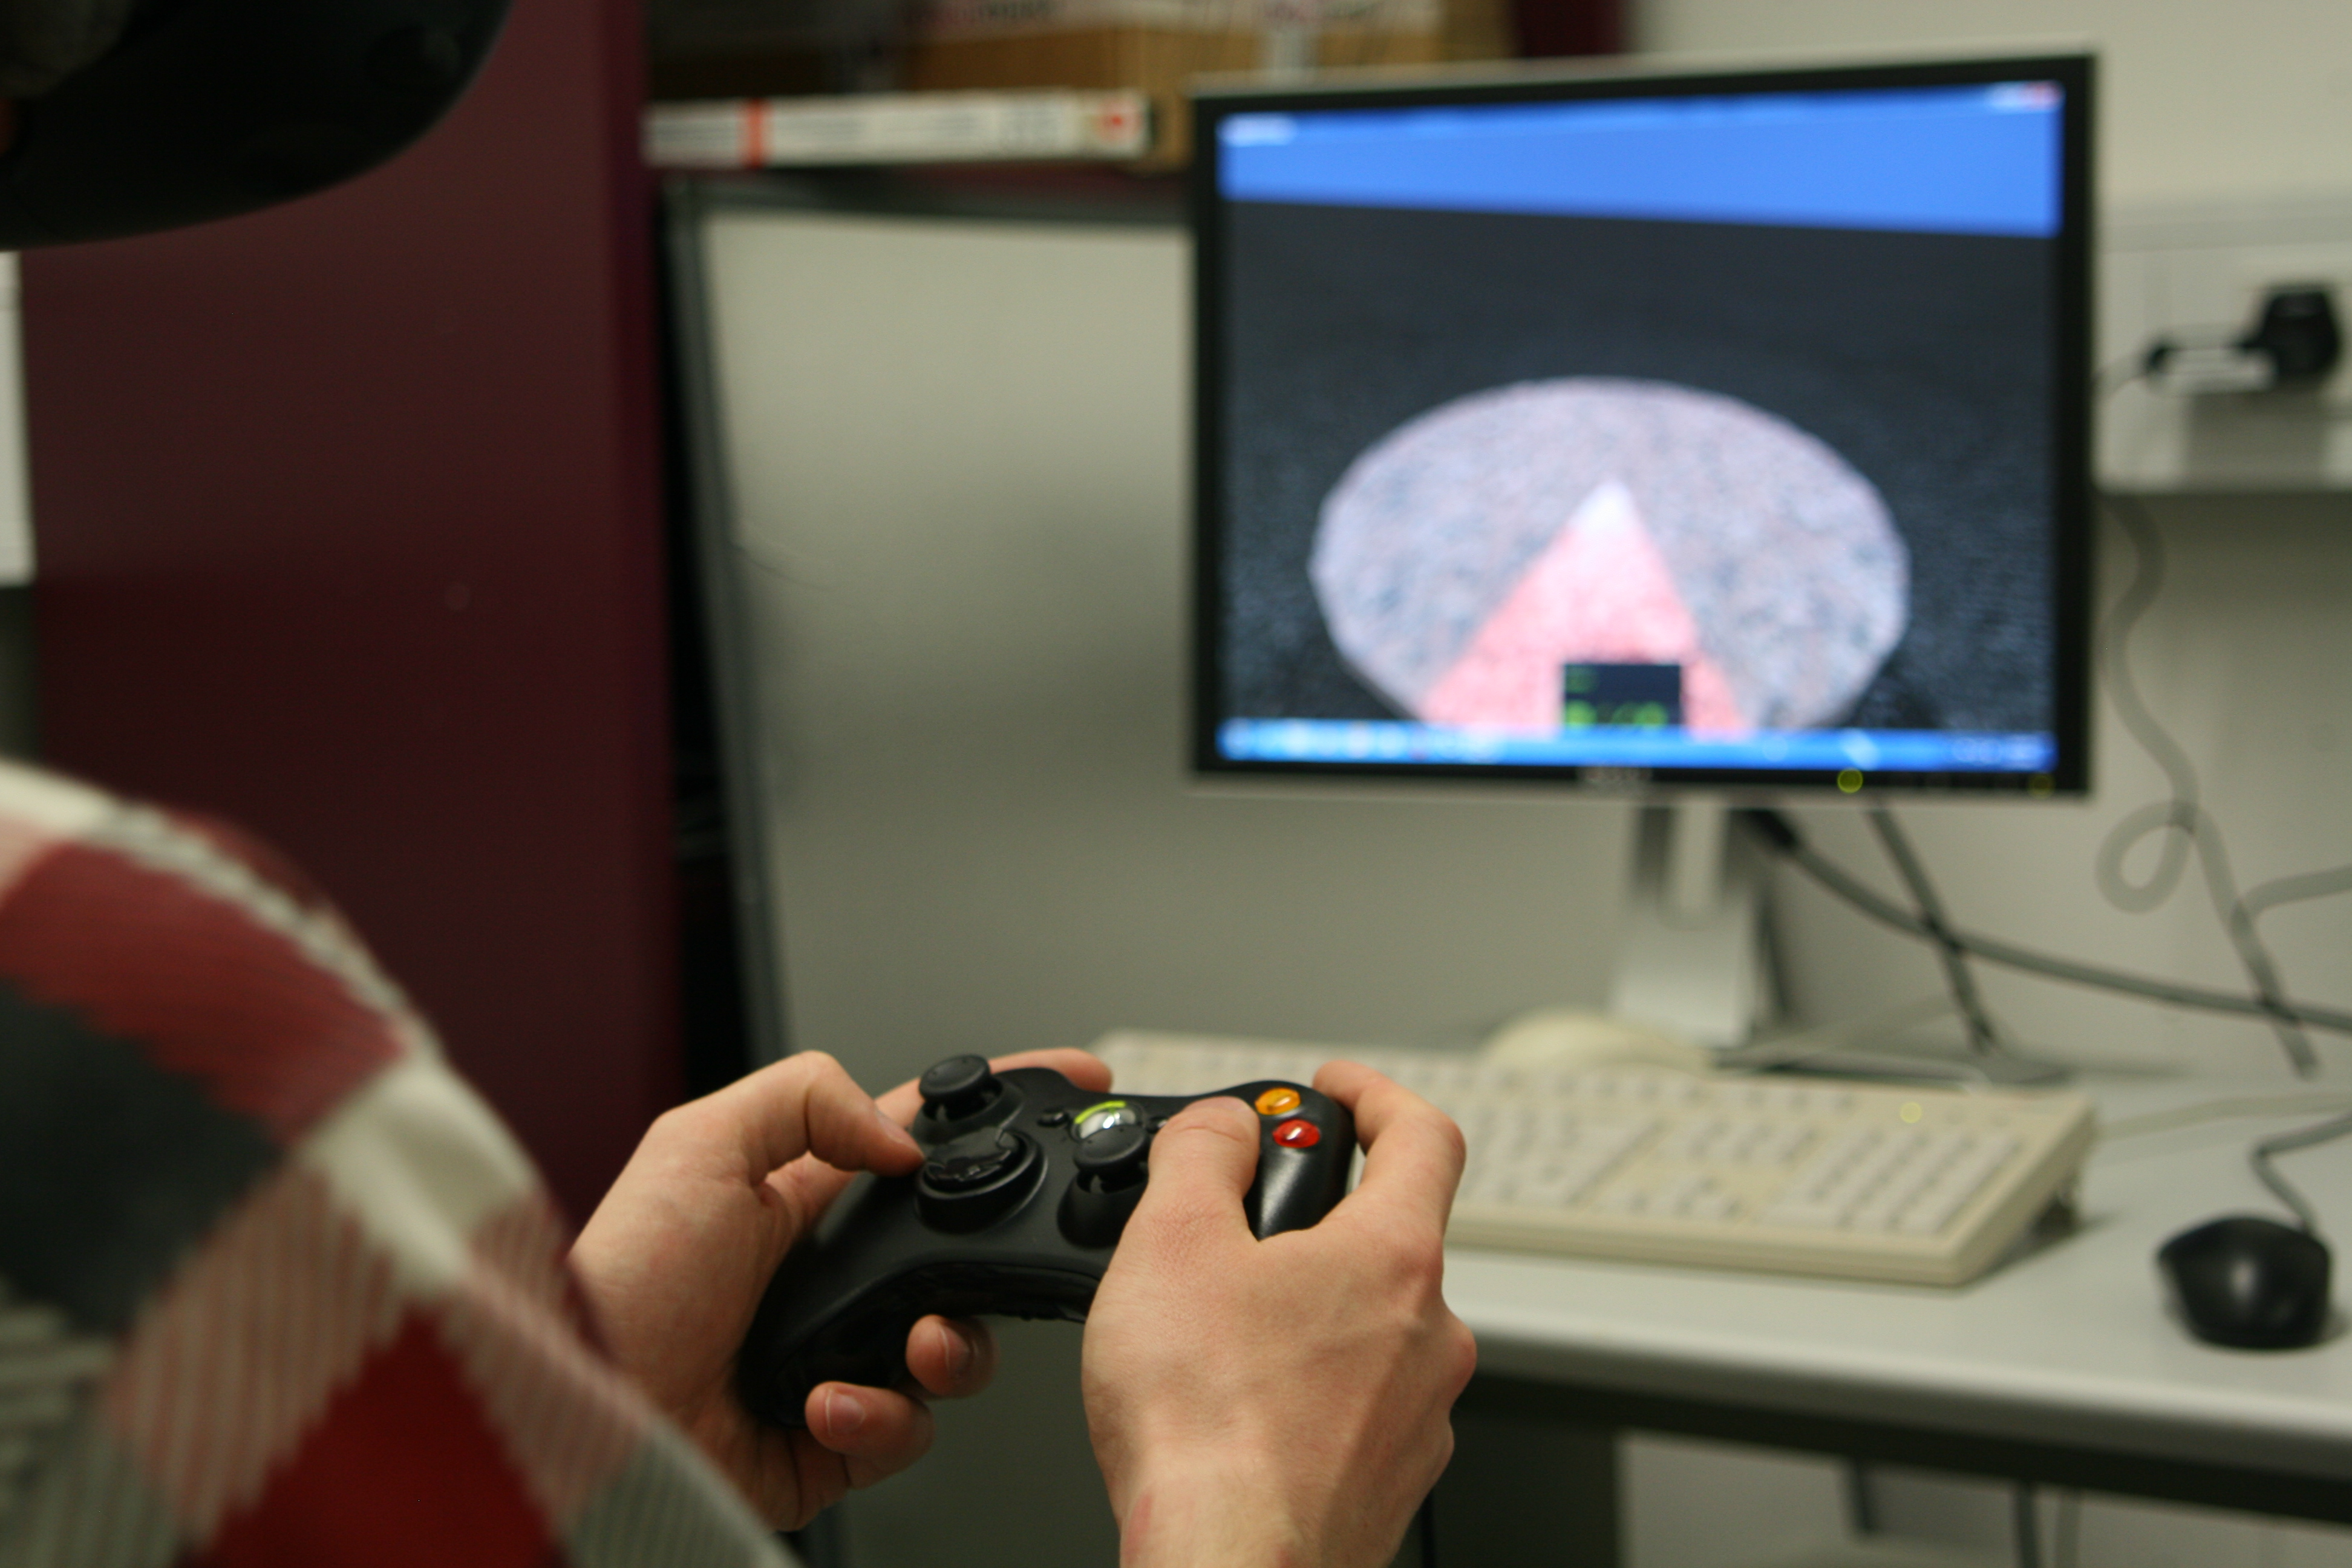
\includegraphics[width=0.5\textwidth]{xbox}
  \caption{XBox controller used to make decisions in the trial phase.} 
  \label{fig:xbox}
\end{subfigure}%
\begin{subfigure}{.5\textwidth}
  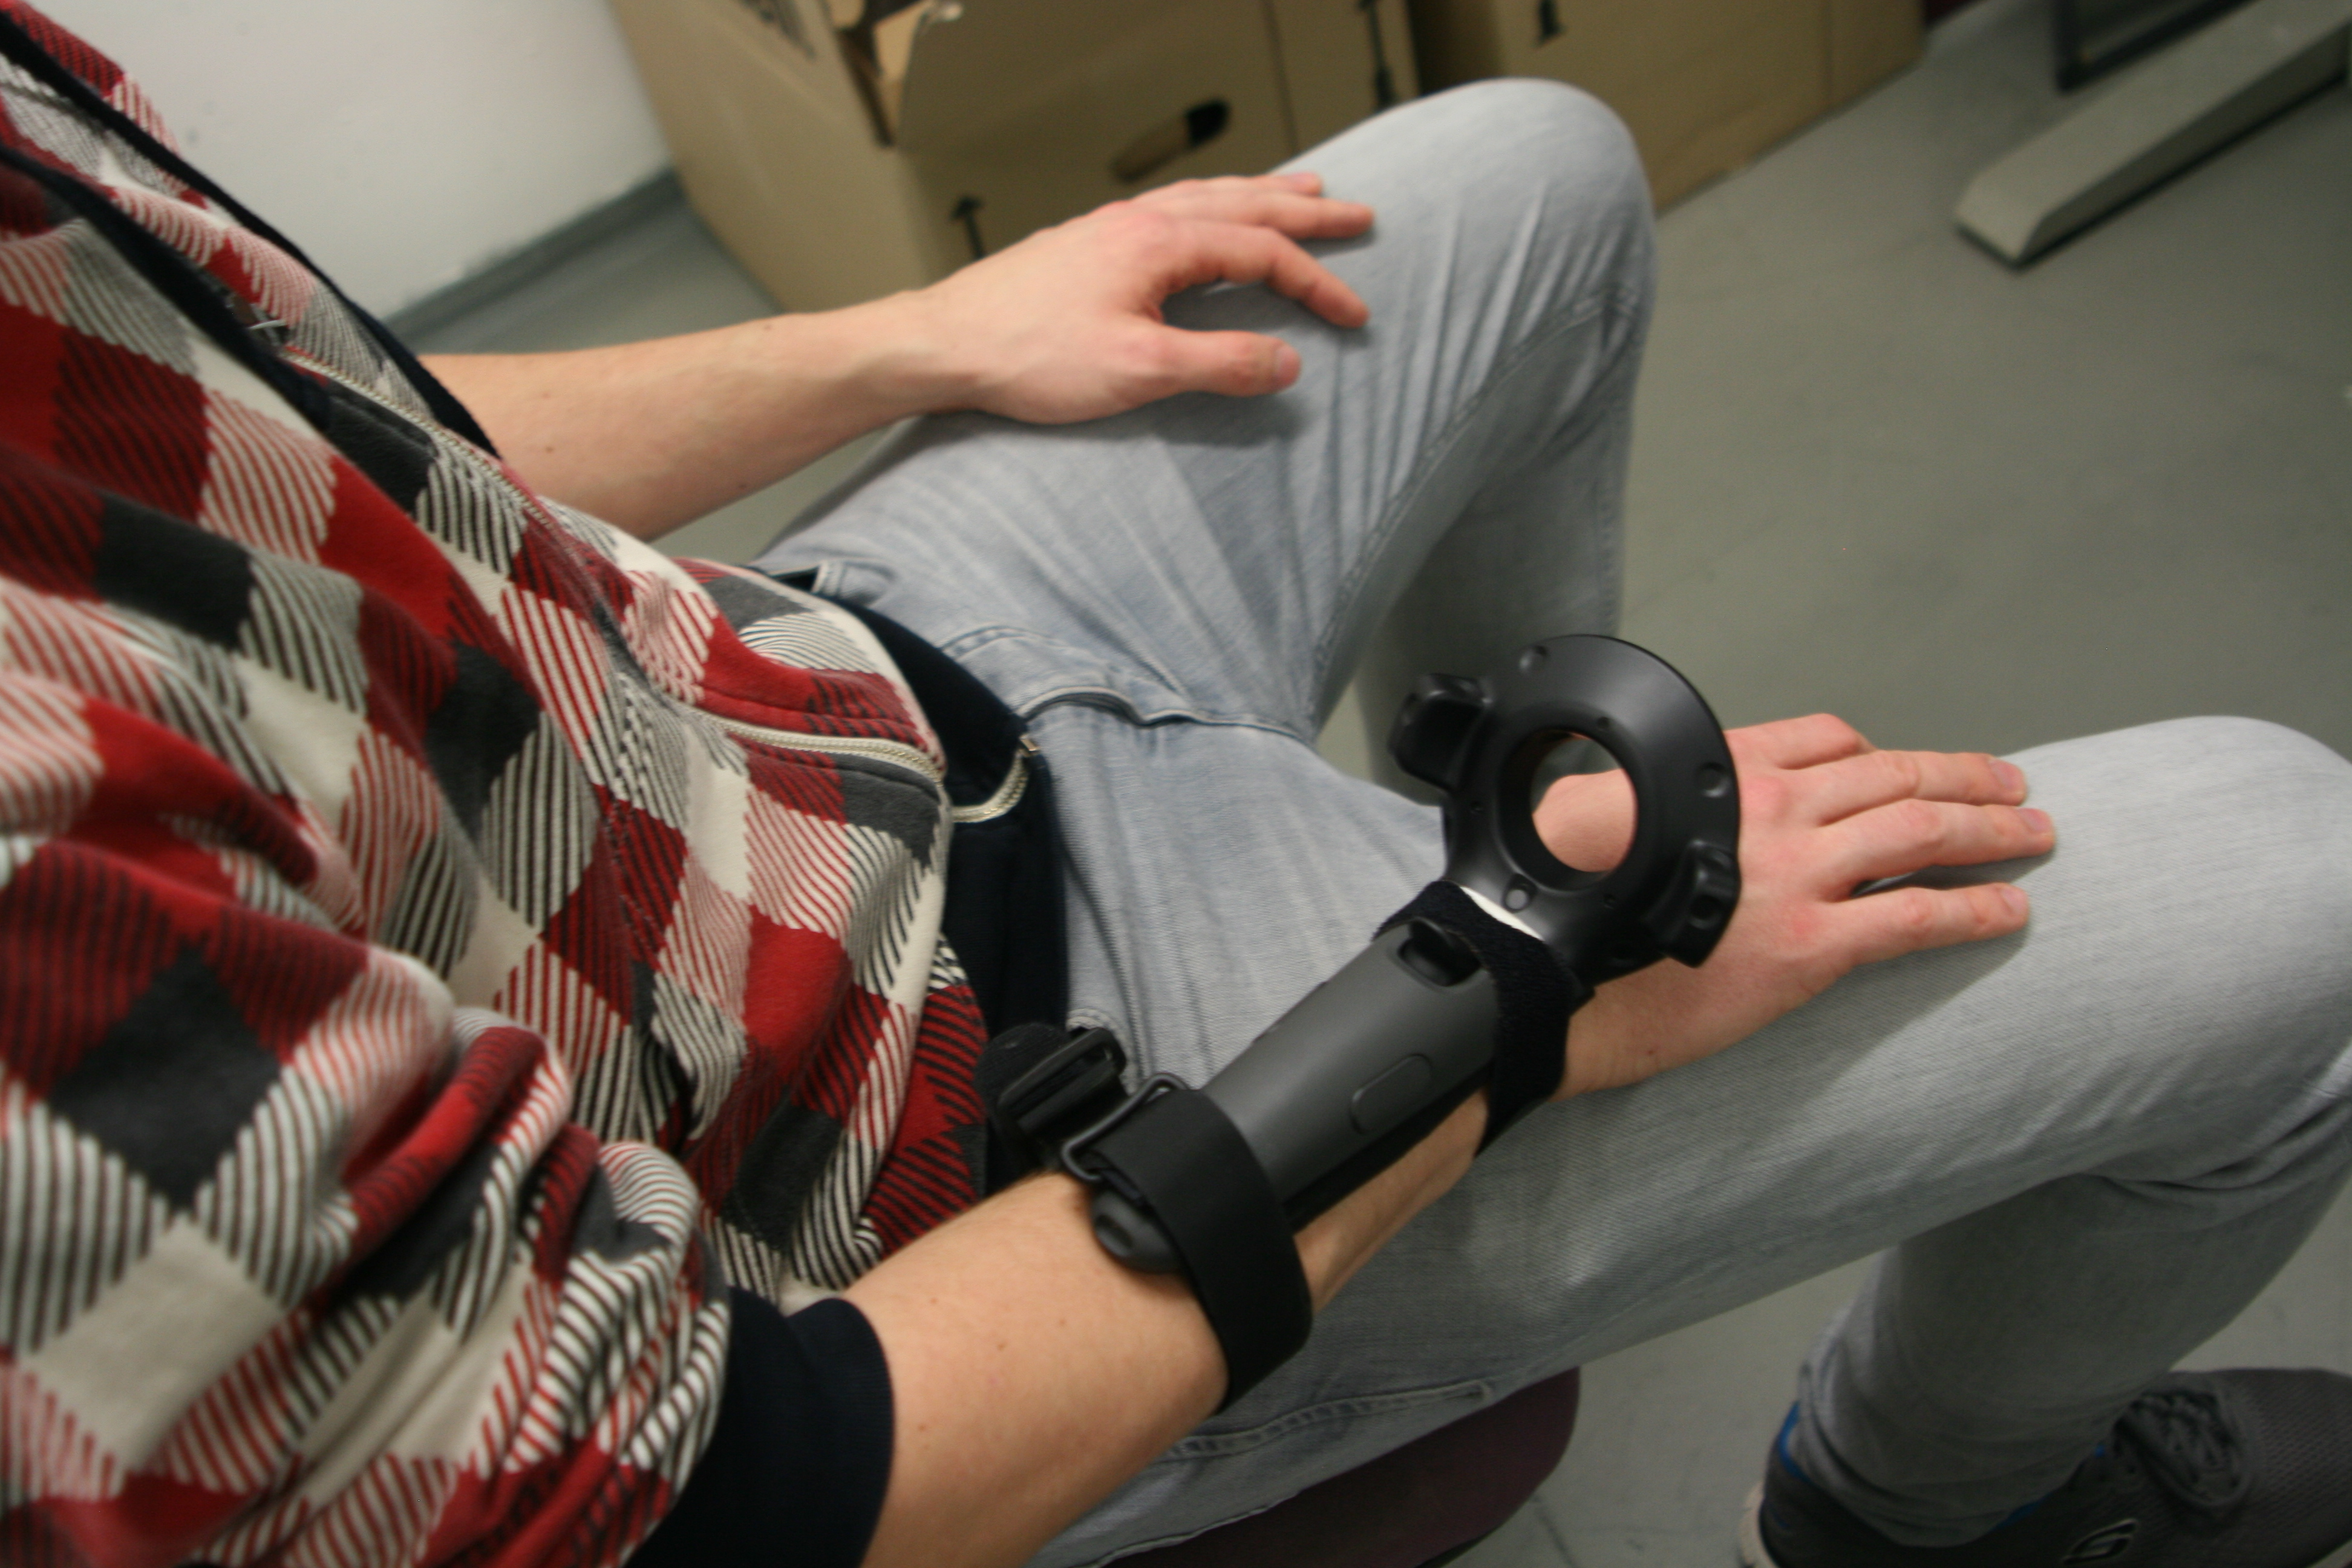
\includegraphics[width=0.5\textwidth]{controller_attach}
  \caption{HTC Vive controller attached to the participant's arm to track hand and arm movements.}
  \label{fig:controller_attach}
\end{subfigure}%
\end{figure}

\begin{figure}[h]
\centering
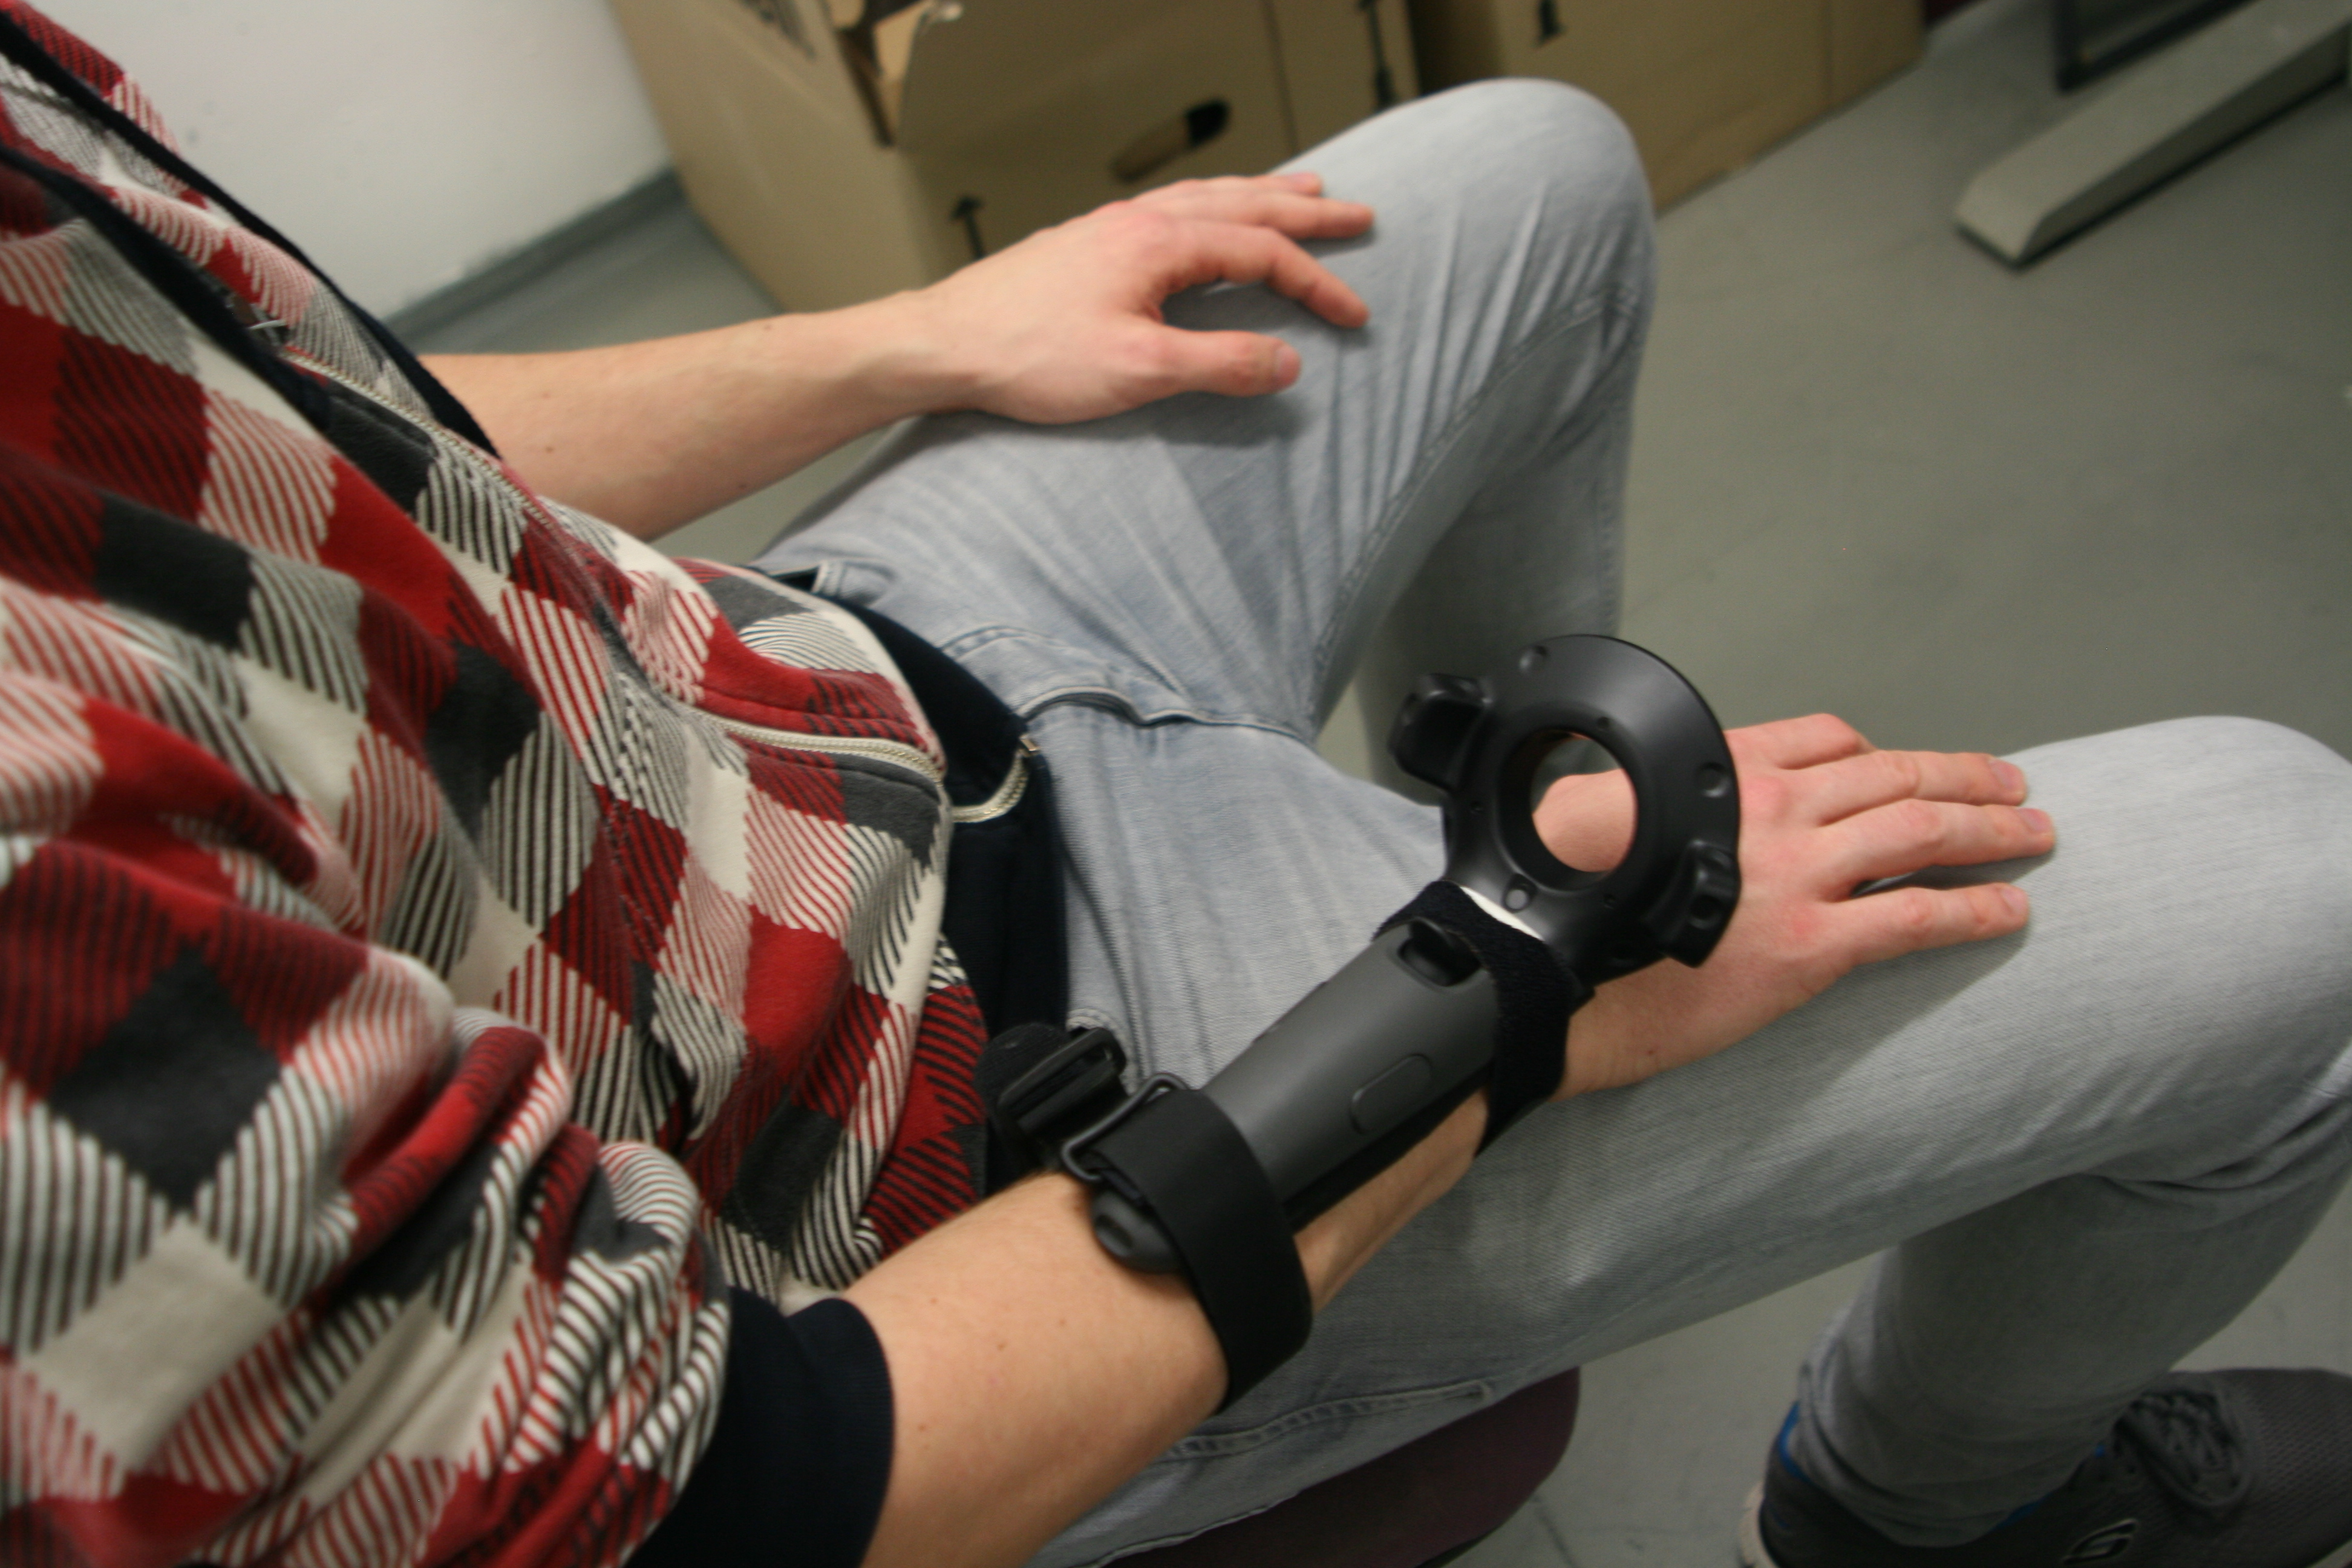
\includegraphics[width=0.5\textwidth]{controller_attach}
\caption{HTC Vive controller attached to the participant's arm to track hand and arm movements.}
\label{fig:controller_attach}
\end{figure}

\begin{figure}[h]
\centering
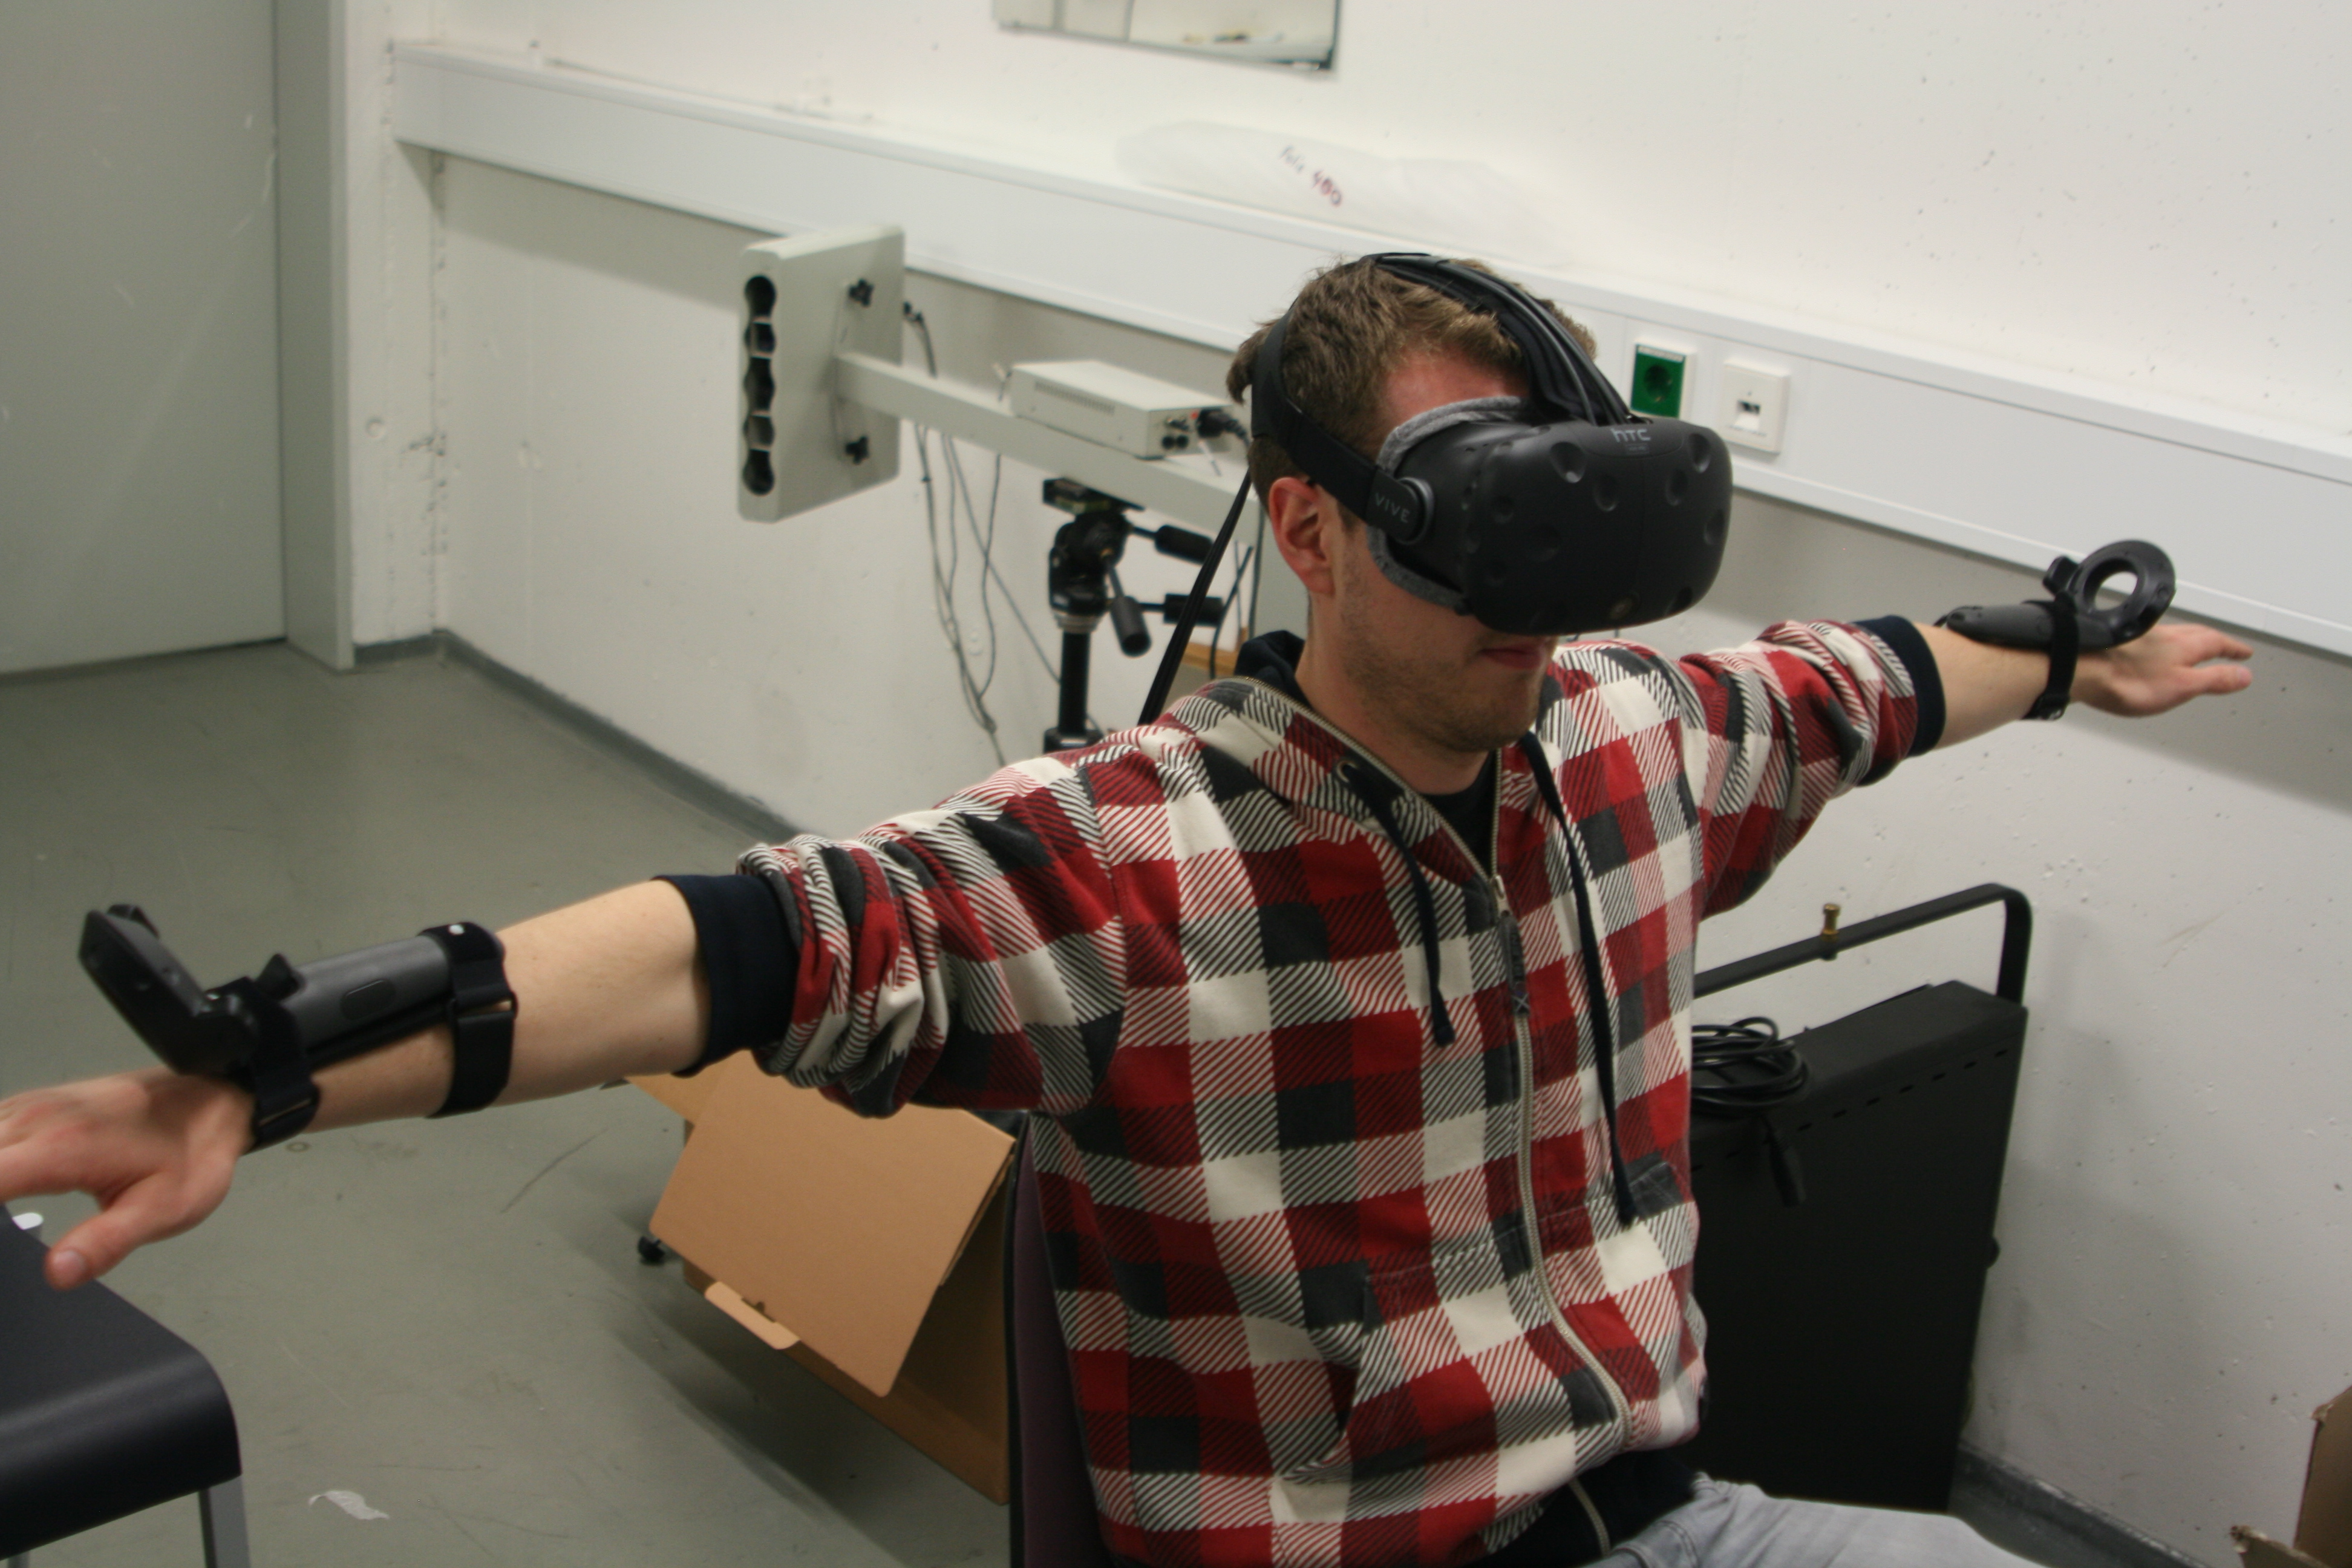
\includegraphics[width=0.5\textwidth]{controller_calibration}
\caption{Two HTC Vive controller attached to the participant's arms to measure and calibrate the virtual arm.}
\label{fig:controller_attach}
\end{figure}

\begin{figure}[h]
\centering
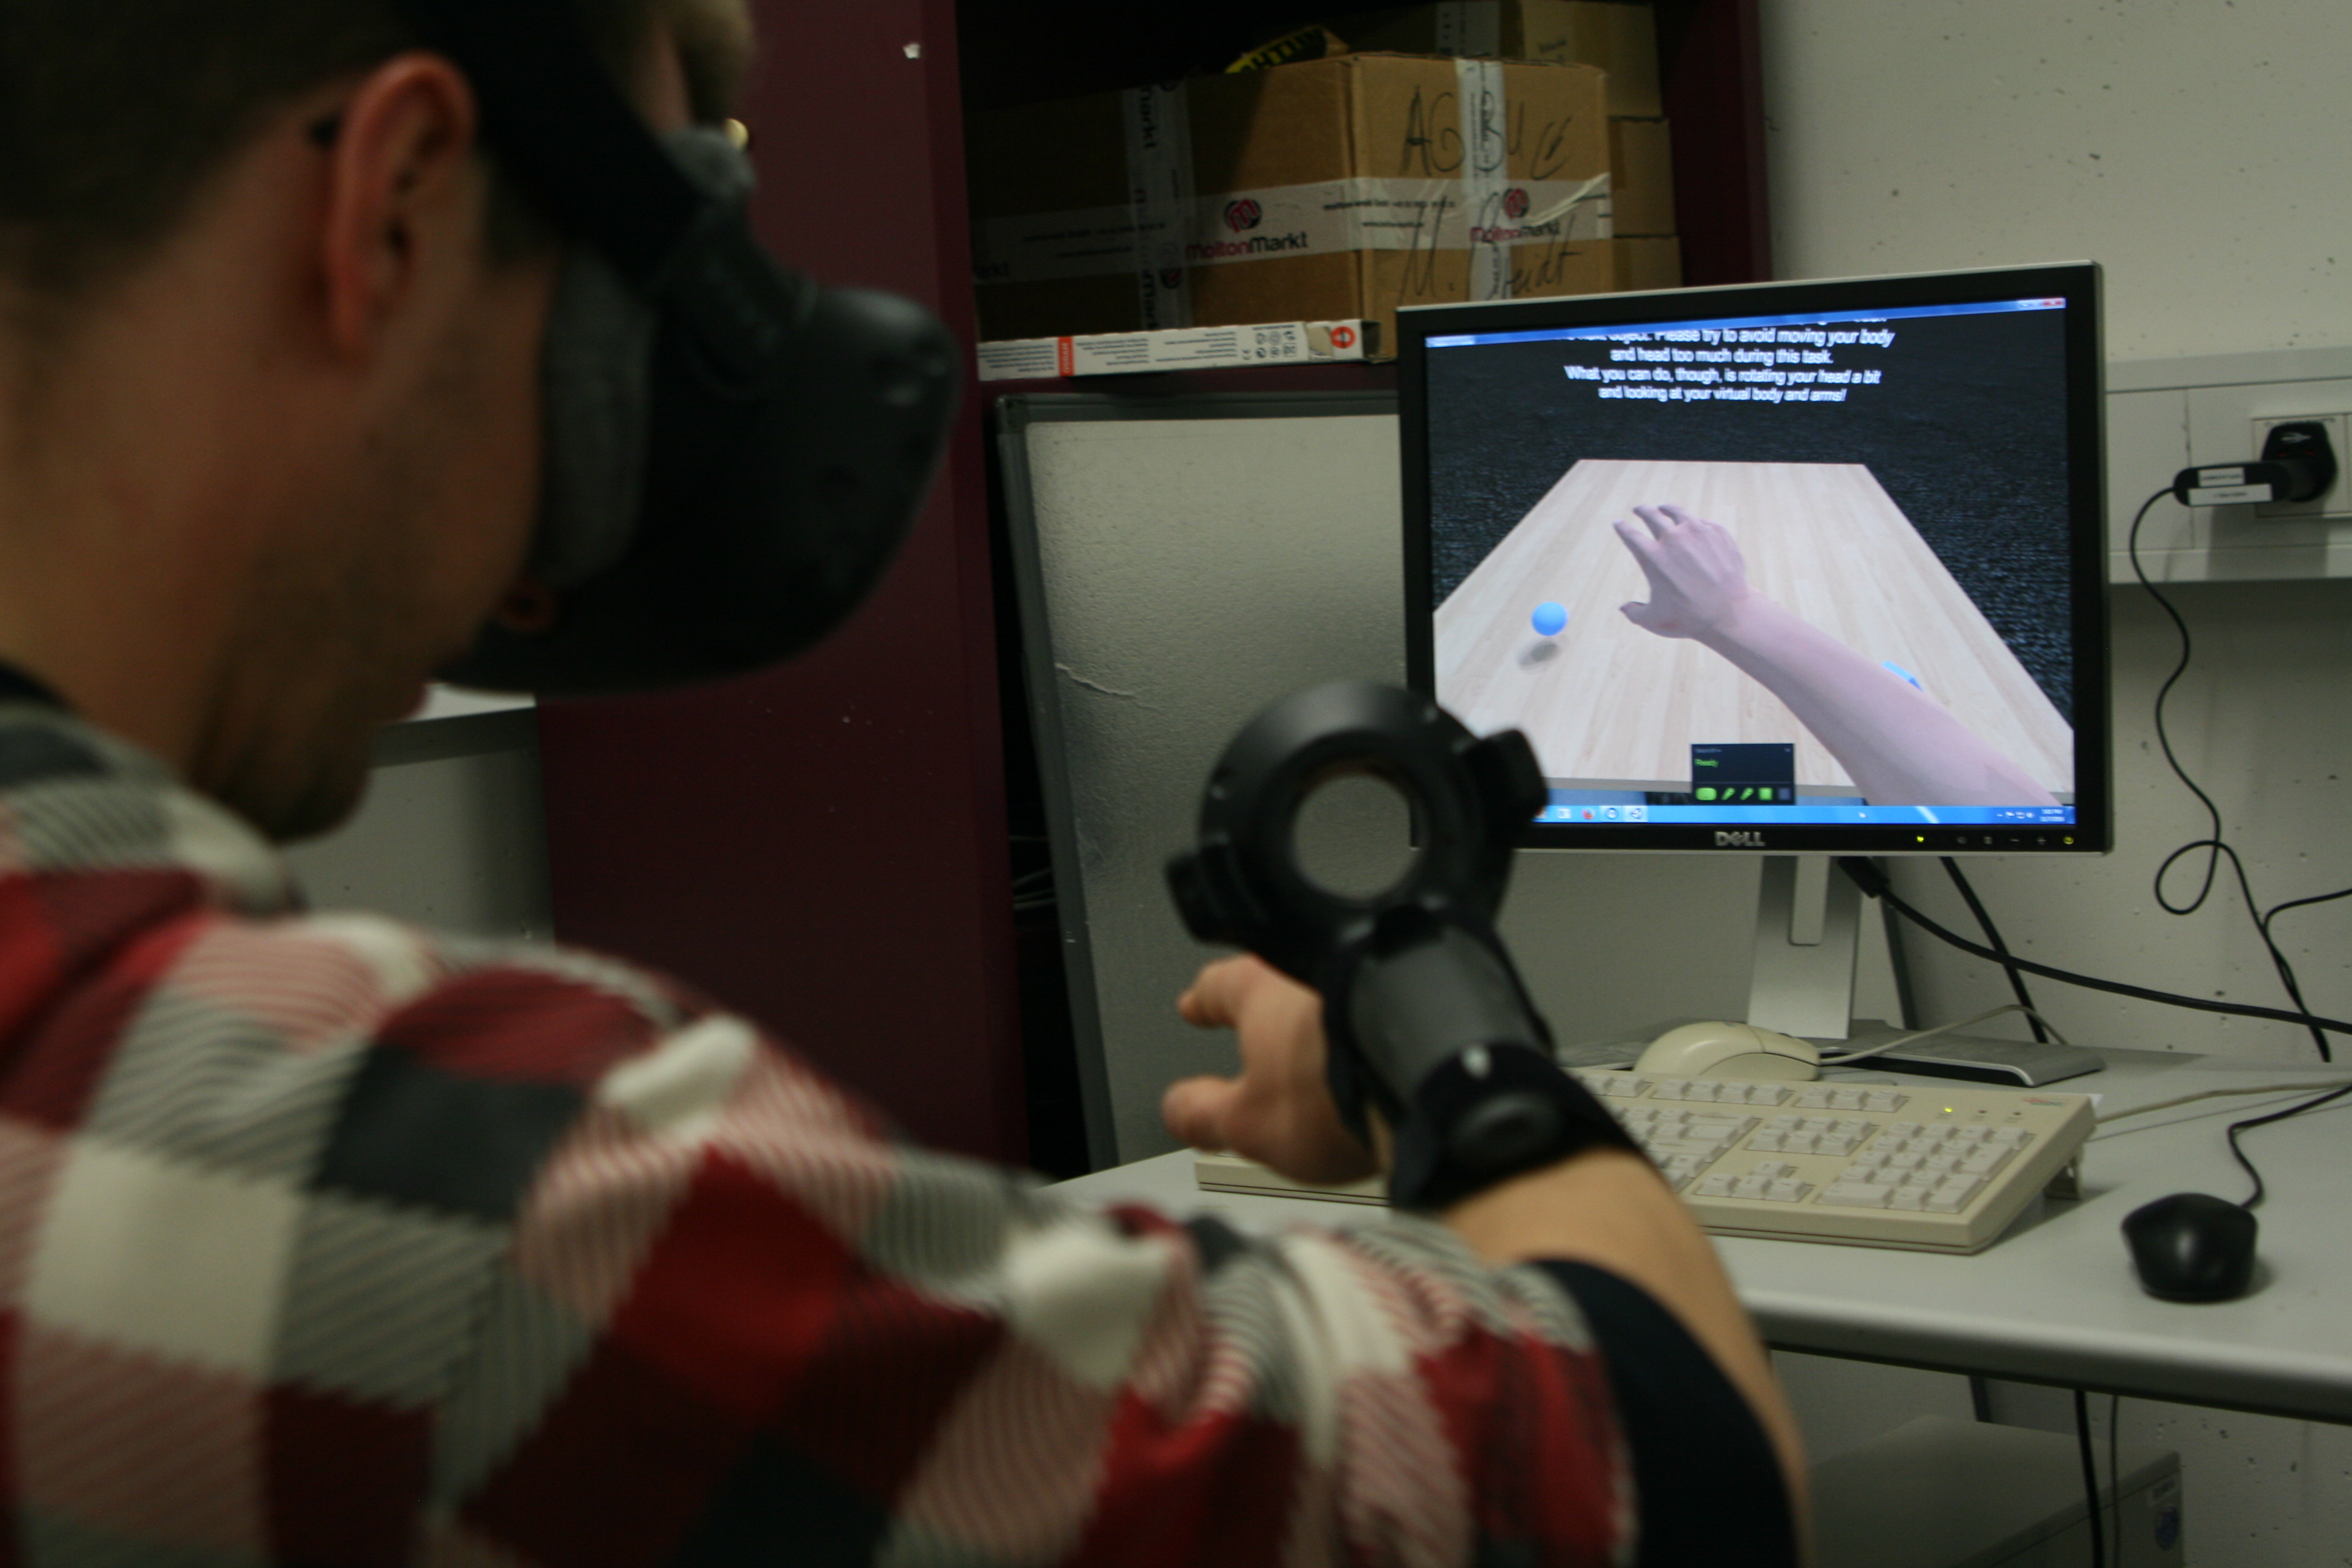
\includegraphics[width=0.5\textwidth]{controller_use}
\caption{HTC Vive controller in use during the adaptation phase. Participants can control the virtual arm with their own hand and arm movements.}
\label{fig:controller_attach}
\end{figure}

\newpage

\subsection{Procedure}
Participants were invited as a group of two people and did not know each other. In one group session the two participants solved the task on their own in a separate virtual environment and together in the same virtual environment. The sequence of single and collaborative condition was counter balanced among all groups. In both the single and collaborative condition participants solved 20 tasks of which all had the same design as described above and differed only in color. In the single condition participants viewed the task always from the same perspective, which means that the starting cube was always placed at the same position in the solution space.
In the collaborative condition we rotated the solution space after 10 trials, which means the starting cube is on one participant's side for the first 10 trials and on the other participant's side for the remaining 10 trials. 

The detailed procedure for the single condition will be explained in the following:
After having read the instructions of the task participants also received a verbal instruction by the experimenter. Before the actual 20 trials began participants had to solve 4 training trials in order to verify that the participant understood the task and the way it has to be solved. It was emphasized that it is important to always stick to the sequence of putting in and removing cubes as described above. Furthermore participants could experience that the starting cube can not be removed and is the only cube in the experiment that collides with the other cubes (that was important to prevent other cubes from overlapping with the starting cube). Participants could also get used to the fact that the top color is always white and the bottom color is always black and that gray always faces to the inside of the solution space. The training trials could be started by the participant by holding a controller button for 2 seconds. When they started the training they saw the solution space surrounded by the 9 cubes which are all in reaching distance. They also saw the starting cube already being placed into the solution space. Above the task participants could see in which trial they currently are. In this case they would see "Training 1/4". Once they have finished a trial they can proceed with the next trial by pressing the controller button again for 2 seconds. 

Before the actual 20 trials started the experimenter repeated the most important instructions. Participants should try to solve the task as quickly and as accurately as possible. Furthermore they were not allowed to move around the problem space and should stay mostly stationary in their position with only a few steps to the sides allowed.
After the 4 training trials participants could start the actual trials as soon as they were ready by clicking a controller button again for 2 seconds. For the actual trial the experimenter would emphasize that participants should always make sure their solution is correct before proceeding with the next task. In case participants did not correctly solve a task and still proceed with the next task the experimenter took notes in order to exclude the trial from the analysis.

The procedure for the collaborative solving of the task was mostly the same. The only difference was that just one participant was able to skip to the next trial and therefore the instructions were that participants had to agree on when to proceed with the next task.

%what needs to go in here is:

%instructions that were given to the participants
%training phase (how many trials...)
%counterbalance single / multi (counterbalanced - 10 each side)
